% !TeX document-id = {d7bfea81-c3f6-4000-b3a4-ebfa033e41d4}
% !TeX root = ./main.tex
% !TEX program = pdflatex
% !BIB program = biber
% !TEX encoding = UTF-8 Unicode
% !TEX options = --shell-escape -synctex=1 -interaction=nonstopmode -file-line-error "%DOC%"
\documentclass[final]{kuee_en}
\usepackage[titletoc]{appendix}
\usepackage{titlesec}
% \titleformat{\chapter}[hang] 
% {\normalfont\huge\bfseries}{\chaptertitlename\ \thechapter}{1em}{} 

% citation
\usepackage[final,breaklinks=true]{hyperref}
\renewcommand*{\sectionautorefname}{Section}
\renewcommand*{\chapterautorefname}{Chapter}
%\renewcommand*{\equationautorefname}{Eqn.}
% \usepackage{cleveref}

\usepackage{pdflscape}

\usepackage{siunitx} % SI units
\sisetup{detect-all}
\usepackage{amsfonts}
\usepackage{amssymb}
\usepackage{xcolor,graphicx}
\usepackage{subcaption}

\usepackage{setspace}
%\singlespacing
%\onehalfspacing
\setstretch{1.1}

\usepackage{sectsty} % change section style
%\allsectionsfont{\sffamily\bfseries}
%\sectionfont{\noindent\textsc} % indent setting

% \usepackage{paralist}
% \usepackage{booktabs}
%\usepackage{fancyhdr}

\usepackage[utf8]{inputenc}
\usepackage[T1]{fontenc}
\usepackage{mathptmx}
%\usepackage{newtxtext, newtxmath}
%\usepackage{tgbonum}

% svg insert
\usepackage[inkscape=on]{svg}
\svgpath{{imgs/svg/}}
\usepackage[off]{svg-extract}
\svgsetup{%
	extractpath=./imgs/svg-extract/,
	inkscapepath=./imgs/svg-inkscape, 
	clean=true,
	convertformat={png},
	convertdpi={png=600},%
	convertdpi=300}

% using modern biblatex
\usepackage[sorting=none,
    backend=biber,
    bibencoding=utf8,
    block=space,
%    style=ieee,
    bibstyle=nature_kuee,
    citestyle=numeric-comp,
    doi=false,isbn=false,url=false,eprint=false]{biblatex}
\bibliography{library}
\bibliography{bibsupple}


% Please add the following required packages to your document preamble:
\usepackage[normalem]{ulem}
\useunder{\uline}{\ul}{}

%%%%%%%%%% Start TeXmacs macros
\newcommand{\mathd}{\mathrm{d}}
\newcommand{\tmname}[1]{\textsc{#1}}
\newcommand{\tmop}[1]{\ensuremath{\operatorname{#1}}}
\newcommand{\tmtextit}[1]{{\itshape{#1}}}
\newcommand{\nosymbol}{}
\newcommand{\tmmathmd}[1]{\ensuremath{#1}}
%%%%%%%%%% End TeXmacs macros

\newcommand\mycaption[2]{\caption[#1]{\textbf{#1}. #2}}
\newcommand{\dint}{D_\mathrm{int}}
\newcommand{\dispu}{ps/km$ \cdot $nm}
\newcommand{\um}{\si{\um}~}
\newcommand{\uW}{\si{\micro\watt}~}
\newcommand{\tbe}{\color{red} To be edited}

\etitle{Broadband frequency entangled photon generation using silicon nitride ring cavities}
% \title{\cjk{窒化シリコンリング共振器を用いた\\広帯域周波数もつれ光子生成}}
\title{Broadband frequency entangled photon generation \\using silicon nitride ring cavities}
\eauthor{Zhenghao Yin} 
\author{\cjk{殷 政浩}}
\supervisor{\cjk{竹内 繁樹 教授}}
\school{\cjk{京都大学大学院工学研究科}}
\depart{\cjk{電子工学専攻}}
\date{\cjk{令和2年1月31日}}

\begin{document}
\maketitle

\begin{abstract}
Frequency entangled photon source is widely required in a variety of optical quantum technology, including but no limited to quantum key distribution, cluster state quantum computation and quantum metrology etc. In the recent decade, chip-scale entangled photon source has been developed in silicon platform for its robustness, large scalability and COMS technology compatibility. However, due to the intrinsic two-photon absorption and limitation of transparency range, the high-intensity and broadband frequency entangled photon pairs such as one-octave, remains an outstanding challenge.

Here, we report the generation of frequency entangled photon pairs using silicon nitride ring cavities, which is transparent from visible to mid-infrared range and no intensity-dependent absorption.
The device design technique is first introduced in the term of phase matching condition. 
Then, we demonstrate the standard subtractive fabrication and compare mainstream silicon nitride deposition methods.
Based on the device transmission, the dispersion evaluation method for broadband frequency entangled photon generation is developed.
The quality factor of \num{5d4} is achieved in our device, promising to generate broadband frequency entangled photons in the optical communication band. 

Furthermore, we exploit fabless device and success to realize chip-scale frequency entangled photon generation at \uW power level. The estimated photon pair generation rate is 15 cps/\uW based on our setup. Furthermore, maximal 46 mode pairs are observed using 24.5 mW pump power, indicating a 106 nm span frequency correlation.


\end{abstract}

\tableofcontents

% !TeX root = ../main.tex
\chapter{Introduction}
% Quantum mechanics has not only boosted up the modern science and technology in different disciplines, but also established the cornerstone for future quantum information processing technology. Furthermore, differing from the past applications, which only involves the quantization nature, the quantum information processing, including but not limited to  quantum computation, quantum communication and quantum metrology, exploits the deep-level physics of quantum mechanics, such as quantum superposition and quantum entanglement.

% Meanwhile, 
The flying qubit---photon---featuring the advantages of long coherent time and multiple degrees of freedom (DoF), is a promising candidate in quantum computation and quantum communication. However, in the term of DoF, much of research up to now focuses on the photon polarization and path entanglement realization, very little attention has been paid to the role of frequency entanglement, which is continuous and infinite in hilbert space. 

Furthermore, the previous research shows that frequency entangled photon pairs can be exploited not only in wavelength division multiplexing quantum key distribution \cite{Wengerowsky2018} but also transferring quantum information in future quantum networks \cite{Tchebotareva2019}. Besides, in recent applications of quantum metrology, quantum optical coherent tomography (QOCT), the broadband frequency entanglement \cite{Okano2015} is also required. 

\section{Background}

% The state-of-art method to generate frequency entangled photon pair is to use bulky crystals.
Compared with crystal experiments, a chip-scale photon source has the advantages of scalability and robustness. A conventional material candidate is silicon on insulator (SOI), since it is CMOS-compatible and supplied by a lot of wafer manufacturers. However, suffering from two photon absorption and stimulated Raman scattering, silicon is no able to generate broadband frequency conversion. Since that, silicon nitride, which is transparent from visible to near infrared range, is preferred to perform broadband frequency entanglement. A recent record is single pair from visible to telecom band \cite{Lu2016}.

\section{Objective}
In the platform of silicon nitride, we utilize the third-order optical nonlinearity and confine the light in the sub-micron scale---optical waveguides. To enhance the nonlinear interaction, we define the ring resonator and couple the light inside along with a bus waveguide. The broadband property is ensured by carefully optimizing the device geometry to achieve a broadband phase matching condition. All the photon pair generation events are detected by single photon detectors and verified by the coincident counting.

In this dissertation, the terms 'broadband photon pair' is used to describe that pairs are generated in different frequency pairs simultaneously and but entangled only in the single mode pair. 

\section{Outline}
The following chapters are sequentially divided in different topics.

% !TeX root = ../main.tex

\chapter{Principal theory}

The way how light travels in a chip-scale is remarkably different the way in free-space. In the sub-micron scale, the electromagnetic wave can only propagate in a fewer cycles due to the constraint of material boundaries. However, since atoms and molecules are much smaller, the refractive index is not changed, as well as the reflection, interference and diffraction. 

Based on these facts, in order to perform quantum optics experiments \textit{at the bottom}, first, we shall confine the light propagation in a specific waveguide. On the other hand, thanks to modern laser technology, nonlinear optics is involved and give birth to optical frequency conversion. To enhance these nonlinear optical phenomena, we adopt the cavity structure and achieve sizable control.

In this chapter, we briefly introduce the guided wave theory and then move the cavity structure, ring resonators. Next, the nonlinear optics, in particular third-order nonlinear processes, is discussed in the following section. Although the quantum nature of photon pair generation distinct from the classical theory, all the physics mentioned above are necessary to analyse our essential research object, the silicon nitride ring resonators.


\section{Guided-wave optics}\label{sec:guide}

In an ideal optical waveguide, the core layer and the cladding layer are usually composed of two different materials, where the refractive index is larger in the core. As an analogue of optical fibers, only in the higher index region can the light propagate, and meanwhile dissipate in a wavelength scale in the lower index region.

Usually, we assume the core and the cladding layer are made of nonmagnetic (magnetic permeability $\mu = \mu_0$) and dielectric material (conductivity $\sigma = 0$). Furthermore, we neglect the nonlinear response of the polarization of electric field ($\vb{P} \simeq \varepsilon_0 \chi \vb{E}$).

Since the waveguide in numerous research objects, is deposited or sputtered using chemical or physical methods, the uneven density in the waveguide layer can not be negligible. Hence, the propagation equation derived from Maxwell's equation is
\begin{equation}\label{eq:aniso}
  (\nabla_{\perp}^2 + k^2 n^2 - \beta^2) \vb{E} = - (\nabla_{\perp} + i
  \beta \hat{\vb{z}}) (\vb{E_{\perp}} \nosymbol \cdot \nabla_{\perp} \ln
  n^2)
\end{equation}
where $\perp$ denotes the transverse component, $\nabla_{\perp}^2 = \nabla_x^2 + \nabla_y^2$. And $k, n, \beta$ are the wave vector in vacuum, refractive index and propagation constant, respectively. While, with the negligible film anisotripy, \autoref{eq:aniso} can be approximated into
\begin{equation}\label{eq:helm}
  (\nabla_{\perp}^2 + k^2 n^2 - \beta^2) \vb{E} = 0
\end{equation}
This is the normal \textit{Helmholtz equation}, indicating the relation between propagation constant $\beta$ and material refractive index, i.e. \textit{chromatic dispersion}.

Next, the boundary conditions determining the solution to Eqn. \ref{eq:helm}, arise from the Maxwell's equations as well.
\begin{eqnarray*}%\label{eq:bcon}
  \vb{\hat{n}} \cdot (\vb{E}_a - \vb{E}_b) & = & 0 \\
  \vb{\hat{n}} \times (\vb{H}_a - \vb{H}_b) & = & 0
\end{eqnarray*}
which is the continuity condition of both electric and magnetic field at all dielectric material interfaces. Here, $\vb{\hat{n}}$ is the normal direction at the material boundary and the subscript $a, b$ denote different regions.

\subsection{Waveguide modes}
In the case of channel waveguides, the index discontinuity from both vertical and horizontal sides can be decomposed into two sets of independent and complete conditions, i.e. the horizontal boundary condition and vertical boundary condition, with the discontinuity on the waveguide corners neglected. In other words, approximately the equation has two independent partiuclar solutions, which is the mathematical origin of \textit{ transverse electric} (TE) modes and \textit{transverse magnetic} (TM) modes.

\begin{figure}
\centering
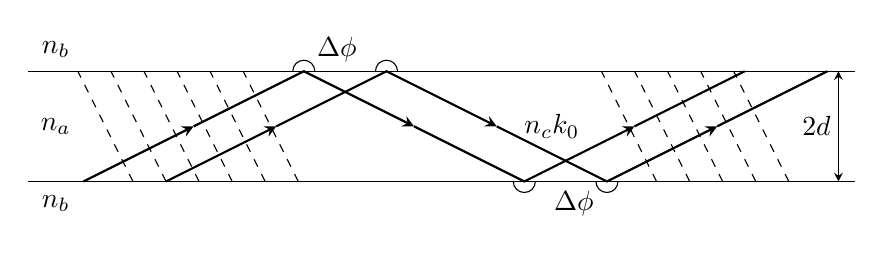
\begin{tikzpicture}[scale=0.7,>=stealth]
\draw (-9,0) -- (6,0) (-9,2) -- (6,2);
% \draw [->] (-9,1) -- (6,1);
\foreach \x in {0,1.5}{
  \draw [thick, ->] (-8+\x,0) -- (-6+\x,1);
  \draw [thick,->] (-6+\x,1) -- (-4+\x,2) -- (-2+\x,1);
  \draw [thick,->] (-2+\x,1) -- (0+\x,0) -- (2+\x,1);
  \draw [thick,-] (2+\x,1) -- (4+\x,2);
}
\foreach \x in {-1,0,1,2,3,4}
	\draw [dashed] (-6.5+0.6*\x,0) -- (-7.5+0.6*\x,2);
\foreach \x in {0,1,2,3,4}
	\draw [dashed] (2.4+0.6*\x,0) -- (1.4+0.6*\x,2);

% \draw [<->] (-9,1.5) --(-9,0.7) -- (-7.4,0.7);
% \draw [->] (-9,0.7) -- (-7.4,1.5);

% \node at (-8.6,1.4) {$\tiny{k_i}$};
% \node at (-8.2,0.4) {$\tiny{\beta}$};
\node at (0.5,1) {$n_c k_0$};

\draw [<->] (5.7,0) -- (5.7,2);
\node at (5.3,1) {$2d$};
\node at (-8.5,1) {$n_a$};
\node at (-8.5,2.4) {$n_b$};
\node at (-8.5,-0.4) {$n_b$};
\node at (-3.4,2.4) {$\Delta\phi$};
\node at (0.9,-0.4) {$\Delta\phi$};

\draw (-3.8,2) arc [start angle=0, end angle=180, radius=0.2];
\draw (-3.8+1.5,2) arc [start angle=0, end angle=180, radius=0.2];

\draw (-3.8+3.6,0) arc [start angle=180, end angle=360, radius=0.2];
\draw (-3.8+5.1,0) arc [start angle=180, end angle=360, radius=0.2];
\end{tikzpicture}
\mycaption{Planar waveguide}{The upper and bottom layer are cladding and the middle is core layer. $\Delta \phi$ represents the Goos-H\"{a}nchen shift at the boundary.}
\label{fig:planar}
\end{figure}

Hence, we can study the eigenequantion by selecting only one set of boundary condition, as used in the \textit{the effective index method}. For example, in a planar waveguide shown in \autoref{fig:planar} ,$\dv*[2]{}{y}=0$\footnote{Since the planar waveguide is infinite at the $y$-direction , thus the solution is identical in arbitrary $xz$-plane, which means no gradient along $x$-axis.},
the TE mode features $E_x=0$ and consider only $y$-component, 
\begin{equation}
    \dv[2]{E_y}{x} + (k^2 n^2 - \beta^2)E_y =0
\end{equation}
and $E_y$ is continous at $x=\pm d/2$, where $d$ is the thickness of core layer.

For the region $|x|>d/2$, the light evanesces at $x$-direction at rate $\kappa$ and in contrast, in the region of core layer, the light performs like stationary wave, denoting with $k_x$. By substituting these conditions, phase continuity is achieved between two interface

\begin{equation}\label{eq:te-eq}
    2k_x d = m\pi + 2\arctan(\kappa/k_x)
\end{equation}
where $m$ is the index of stationary wave. The second term can be treated as the Goos-H\"{a}nchen phase shift. Overall, the waveguide modes characterize that the phase shall maintain itself with an $m\pi$ shift along with the shift at the boundaries.

In the case of TM modes, the eigen equation is 
\begin{equation}\label{eq:tm-eq}
    2k_x d = m\pi + 2\arctan(\delta\kappa/k_x)
\end{equation}
where $\delta=n_a/n_b$ is the index ratio and only differs from \autoref{eq:te-eq} with this parameter. conclusively, the less is $\delta$ parameter, the propagation constant of TE and TM modes are closer.

\subsection{Dispersion relation}
Based on \autoref{eq:te-eq} and \autoref{eq:tm-eq}, $k_x$ can be solved and then utilized to calculate propagation constant $\beta$, since $n_a^2k^2 = k_{\perp}^2 + \beta^2$. In the case of channel waveguides, the TE and TM solutions are both necessary. Therefore, propagation constants $\beta$ can be expressed as the product of free space wave vector $k$ and the \textit{ effective index} $n_{\mathrm{eff}}$
\begin{equation}\label{eq:disp_bk}
    \beta = n_{\mathrm{eff}}k = n_{\mathrm{eff}}(\lambda) \frac{2\pi}{\lambda} = n_{\mathrm{eff}}(\omega) \frac{\omega}{c}
\end{equation}
along with the differential form
\begin{align}\label{eq:ng-def}
    \dv{\beta}{k} &= n_{\mathrm{eff}} + k \dv{n_{\mathrm{eff}}}{k} = n_{\mathrm{eff}} - \lambda\dv{n_{\mathrm{eff}}}{\lambda} \equiv n_g \\
    \dv{\omega}{\beta} &= c \dv{k}{\beta} = \frac{c}{n_g} \equiv v_g  
\end{align}
which defines the group index $n_g$ and group velocity $v_g$.

This formula linking $\beta - k$ or $\beta - \omega$ is named as dispersion relation, which gives the physics that light with different color propagates at different \textit{speed}. Furthermore, \autoref{eq:te-eq} and \autoref{eq:tm-eq} also indicate that the dispersion relation intrinsically depends on waveguide geometry.

\section{Ring resonators}

The ring resonators comprise of a bus waveguide and a ring waveguide, are usually demonstrated as optical filters or modulators at a wide range of platforms. The working principle of ring resonator can be derived completely \cite{Bogaerts2012} as an analogue to Fabry-P\'{e}rot etalon, based on the coupling mode theory. 

\begin{figure}
    \centering
	\includesvg{mrr_illus}
	\mycaption{An all-pass type ring resonator}{The transmitted spectrum is filtered periodically by the ring waveguide, in the case satisfying resonance condition.}
    \label{fig:mrr-illus}
\end{figure}

In the model illustrated in \autoref{fig:mrr-illus}, the self-coupling coefficient $\tau$ and the cross-coupling coefficient $\kappa$ can be evaluated analytically or using numerical simulation. Assuming the coupling only occur at the very close area, $\tau,\kappa$ are the power splitting ratios of the coupler and satify $\tau^2 + \kappa^2 =1 $ if the coupling section is lossless. $a$ is the single-pass amplitude transmission, including both propagation loss in the ring and loss in the couplers.

\begin{figure}
    \centering
    \includesvg{mrr_cp}
    \mycaption{The transmission spectrum of a ring resonator}{}
    \label{fig:mrr_spec}
\end{figure}

The transmission rate of a all-pass type ring cavity takes the form of
\begin{equation}\label{eq:trans_phi}
    T = \frac{I_\mathrm{pass}}{I_\mathrm{input}} = \frac{a^2 - 2a\tau \cos \phi + \tau^2}{1 - 2ar \cos \phi + a^2 \tau^2}
\end{equation}
where $\phi=\beta L$ is the phase shift in a single round trip. 

\subsection{Coupling condition}

By plotting the function in \autoref{fig:mrr_spec}, we can see, the extinction ratio of absorption peak is defined by the self-coupling coefficient $\tau$ and the single-pass amplitude transmission $a$ due to device geometric differences, like the gap between the bus waveguide and the ring cavity. Namely, $a$ and $\tau$ both determine the coupling condition, which can be categorized in three cases
\begin{itemize}
    \item \textbf{weak coupling} $a>\tau$. The loss inside the ring is larger than the power coupled from bus waveguides.
    \item \textbf{critical coupling} $a=\tau$. The loss and self-coupling are in balance. The optical power restored in the resonator achieve the minimum.
    \item \textbf{over coupling or strong coupling} $a<\tau$. The coupling is too strong for the light to dissipate in a single round trip.
\end{itemize}

Previous work \cite{Yusuke2017} proposed a method to evaluate the coupling condition above using the experimentally measured device transmission. Considering the loss in the coupler, bent segment of ring and higher mode perturbance, usually the critical coupling varies from modes and the cross section of waveguides \cite{Pfeiffer2017}.

\subsection{Spectrum characteristics}
Meanwhile, the minimum of transmission rate $T$ can be achieved periodically as $\phi=2 m \pi$, which defines the resonance of ring resonators. Therefore, the resonance condition is derived as
\begin{equation}\label{eq:res-con}
    \beta L =2 m \pi
\end{equation}
where $m$ is the mode index. Specifically, the propagation constant $\beta$, shall be an integral times of a quasi wave vector $2\pi/L$. With this condition, the free spectral range (FSR) of wavelength and frequency are obtained
\begin{align}
    \Delta \lambda_\mathrm{FSR} &\approx \frac{\lambda_\mathrm{res}^2}{n_g L} \label{eq:fsr-wl} \\
    \Delta \omega_\mathrm{FSR} &\approx \frac{2\pi c}{n_g L} \label{eq:fsr-w}
\end{align}

In both wavelength and frequency domain, FSR determines the spacing of neighbouring resonant peak. This is a significant factor when the ring resonators are designed.

Furthermore, from \autoref{eq:trans_phi}, the full width at half maximum (FWHM) of the resonance spectrum is derived as $\delta\lambda$
\begin{equation}\label{eq:fwhm_phi}
    \delta\phi = \frac{2(1- a \tau)}{\sqrt{\tau a}}
    % \lambda_{\mathrm{res}}^2
\end{equation}
\begin{figure}
    \centering
    \includesvg{mrr_fsr_illus}
    \mycaption{Illustration of wavelength transmission spectrum of ring resonators}{FSR, free spectral range, the distance between neighbouring resonant wavelength. FWHM, full width at half maximum.}
    \label{fig:my_label}
\end{figure}

Likely, since the phase $\phi$ is related with the wave vector $k$ in \autoref{eq:ng-def}. Substituting $\delta \phi = L n_g \delta k$, the half width of wavelength is
\begin{equation}
    \delta \lambda = \dv{\lambda}{k}\delta k = \frac{\lambda_\mathrm{res}^2}{2\pi L n_g} \frac{2(1- a \tau)}{\sqrt{\tau a}} \label{eq:fwhm_wl}
\end{equation}
the same, at the frequency domain
\begin{equation}
    \delta \omega = \dv{\omega}{k}\delta k = \frac{c}{ L n_g} \frac{2(1- a \tau)}{\sqrt{\tau a}} \label{eq:fwhm_w}
\end{equation}

Note in \autoref{eq:fsr-wl} \autoref{eq:fsr-w} \autoref{eq:fwhm_wl} and \autoref{eq:fwhm_w}, the group index $n_g$ is explicit instead of the effective index $n_\mathrm{eff}$ because both free spectral range and full width depend on the differential form, \autoref{eq:ng-def}.

And the finesse $F$ of the resonator is defined 
\begin{equation}
    F \equiv \frac{2\pi}{\delta\phi} = \frac{\pi\sqrt{\tau a}}{2(1- a \tau)}
\end{equation}

Finally, we define the quality factor, a measure of the sharpness of the resonance relative to its central frequency.

\begin{equation}\label{eq:q-def}
    Q = \frac{\lambda_\mathrm{res}}{\delta \lambda} =  \frac{\pi L n_g \sqrt{\tau a}} {\lambda_\mathrm{res} (1- a \tau)}
\end{equation}

Usually, the \textit{Q}-factor can be decomposed into two parts by formula $Q^{-1}=Q_{i}^{-1} + Q_{l}^{-1}$. And $Q_{i}, Q_{l}$ are intrinsic \textit{Q}-factor and loaded \textit{Q}-factor, referring to the loss inside the ring waveguide and at the coupler, respectively. The physical meaning of the finesse and \textit{Q}-factor relates to the number of round-trips before being lost to internal loss and the bus waveguides when the power is depleted to $1/e$ of its initial value.

\section{Thrid-order nonlinear optics}

Although the nonlinear effect is ignored during the derivation of waveguide modes in \autoref{sec:guide}, 
for numerous materials, the nonlinear response of electric field is significant even at mW level, which is easy to occur with assistance of modern lasers. The origin of nonlinear optic phenomena is similar to the movement of the object in a potential field, such as the ball-spring model. 

In the nonlinear material, the atoms or molecules are driven by the external electric field, due to the around chemical bonds or molecular orientation, the displacement of atoms or molecules perform nonlinear dependence on the strength of field. In real-world materials, interaction coming arising from various frequency leads to the addition or subtraction of these frequency components. This explains the frequency conversion nature in nonlinear optics.

% these phenomena are widely used in quantum optics, such as spontaneous parametric down conversion. And
It is worth mentioning that not only in the bulk crystals, but also in the sub-micron scale \cite{Leuthold2010}, the nonlinear response is still efficient, even over a single-layer two-dimensional material.

% In this section, we prefer to introduce both second-order and third-order optical nonlinearity. 
Here, a brief theoretical derivation is elucidated and in the following part, degenerate four wave mixing is emphasized. In an isotropic nonlinear medium, assuming only instantaneous dielectric response, the relation between the polarization and the electric field is expressed by a power series in the electric field
\begin{align}\label{eq:nlp}
    \vb{P}(t) & = \varepsilon_0 \large (\chi^{(1)}\vb{E}(t) + \chi^{(2)}\vb{E}^2(t) + \chi^{(3)}\vb{E}^3(t)) \\
			& = \varepsilon_0 \chi^{(1)}\vb{E}(t) + \vb{P}_\mathrm{NL}(t)
\end{align}

Note in \autoref{eq:nlp}, the nonlinear susceptibilities $\chi^{(2)}$ and $\chi^{(3)}$ are second-rank and third-rank tensors, corresponding to the tensor product with $\vb{E}^2$ and $\vb{E}^3$. The higher order response is neglected and sequentially, only $\chi^{(2)}$ processes and $\chi^{(3)}$ processes are to be introduced.

\bigskip
\noindent\textbf{$\chi^{(2)}$ processes} 

In centrosymmetric crystals such as silicon, the second-order susceptibility term is absent. However, in other materials like lithium niobate (\ce{LiNbO3}) and aluminium nitride (AlN), the second-order nonlinearity are essential to realize electro-optic modulation and second harmonic generation.

\bigskip
\noindent\textbf{$\chi^{(3)}$ processes} 

Silicon and silicon nitride are both cubic crystal. Due to the third-order dependence, another factor equivalent to the optical intensity is involved, the $\chi^{(3)}$ process is also named as intensity-dependent effect or Kerr effect.

Consider three frequency components of $\vb{E}^3$, using the complex expression of electric field
\begin{equation}
    \vb{E}(\vb{r}, t) = \sum_{k=1}^3 \vb{E}_{\omega_k}(\vb{r}, t) =  \frac{1}{2} \sum_{k=1}^3 \qty ( \vb{E}_{\omega_k}(\vb{r})e^{i\omega_k t} + c.c.)
\end{equation}
\begin{figure}
    \includesvg{energy_diagram}
    \mycaption{Illustration of possible energy diagram in typical third-order nonlinear processes}{}
    \label{fig:energy-level}
\end{figure}
Substituting into third-order term in \autoref{eq:nlp} and arranging with the same propagation direction, the third-order polarization is 

\begin{align}
  \vb{P}^{(3)}(t) 
  & = \frac{3}{4} \varepsilon_0 \chi^{(3)} \left[| \vb{E}_{\omega_1} |^2 \vb{E}_{\omega_1} + \cdots\right] & \mathrm{SPM} \\
  & + \frac{6}{4} \varepsilon_0 \chi^{(3)} \left[(| \vb{E}_{\omega_2} |^2 + |\vb{E}_{\omega_3} |^2) \vb{E}_{\omega_1} + \cdots \right] & \mathrm{XPM} \\
  & + \frac{1}{4} \varepsilon_0 \chi^{(3)} \left[(\vb{E}_{\omega_1}^3 e^{i \omega_1 t} + c.c.) + \cdots\right] & \mathrm{THG} \\
%   \tag{\stepcounter{equation}\theequation}
  & + \frac{3}{4} \varepsilon_0 \chi^{(3)} \left[ \frac{1}{2} (\vb{E}_{\omega_1}^2 \vb{E}_{\omega_2} e^{i (2 \omega_1 + \omega_2) t} + c.c.) + \cdots \right] & \mathrm{FWM} \label{eq:fwm1} \\ 
  & + \frac{3}{4} \varepsilon_0 \chi^{(3)} \left[ \frac{1}{2} (\vb{E}_{\omega_1}^2 \vb{E}^{\ast}_{\omega_2} e^{i (2 \omega_1 - \omega_2) t} + c.c.) + \cdots \right] & \mathrm{FWM} \label{eq:fwm2} \\ 
  & + \frac{6}{4} \varepsilon_0 \chi^{(3)} \left[ \frac{1}{2} (\vb{E}_{\omega_1} \vb{E}_{\omega_2} \vb{E}_{\omega_3} e^{i (\omega_1 + \omega_2 + \omega_3) t} + c.c.) + \cdots \right] & \mathrm{FWM}  \label{eq:fwm3} \\
  & + \frac{6}{4} \varepsilon_0 \chi^{(3)} \left[ \frac{1}{2} (\vb{E}_{\omega_1} \vb{E}_{\omega_2} \vb{E}^{\ast}_{\omega_3} e^{i (\omega_1 + \omega_2 - \omega_3) t} + c.c.) + \cdots \right] & \mathrm{FWM} \label{eq:fwm4}
\end{align}

In above equations, $\cdots$ stands for all possible permutation terms contributed by frequencies $\omega_1, \omega_2, \omega_3$. The abbreviation on the right side represent for 

\bigskip
\noindent\textbf{SPM, self-phase modulation}

SPM adds an intensity-dependent term except the linear polarization, leading to a broadening of the pulse spectrum.

Note the $\chi^{(3)}$ is complex, thus the imaginary part may contribute to another intensity-dependent absorption mechanics, which is usually depicted in the \textit{two-photon absorption} (TPA). The free carriers excited by TPA in further change the temporally both the absorption coefficient and the refractive index of material.
\begin{equation}\label{eq:spm-index}
    n = n_0 + n_2 I + i \frac{\lambda}{4\pi}(\alpha_0 + \alpha_2 I)
\end{equation}
where the $I$ is the intensity, $n_2$ is the Kerr coefficient and $\alpha_0, \alpha_2$ are related with TPA-induced free carrier absorption (FCA) and free carrier index (FCI) change, both interrelated with third-order susceptibility
\begin{align}
    n_2     &= \frac{1}{cn_0^2\varepsilon_0} \frac{3}{4} \Re{\chi^{(3)}} \\
    \alpha_2&= \frac{-\omega}{c^2n_0^2\varepsilon_0} \frac{3}{2} \Im{\chi^{(3)}}
\end{align}
A figure of merit (FOM) is often used to compare the magnitude of Kerr coefficient $n_2$ with the strength of the TPA coefficient $\alpha_2$
\begin{equation}
    \mathrm{FOM} = \frac{1}{\lambda} \frac{n_2}{\alpha_2}
\end{equation}

\bigskip
\noindent\textbf{XPM, cross-phase modulation} 

XPM can be seen the first signal index influenced by a second signal. And the coeffiecient of XPM is twice as strong as the SPM coefficient.

\bigskip
\noindent\textbf{THG, third-harmonic generation} 

Like SHG, THG generated a new frequency with is one-third of input frequency. 

\bigskip
\noindent\textbf{FWM, four wave mixing} 

% \item DFWM, degenerate four wave mixing
% Another factor to mention is that the coefficient in each $\chi^{(3)}$ process arises from the combination of three frequency components. For instance, on the numerator \autoref{eq:def-dfwm} has the factor 3 but \autoref{eq:def-ndfwm} has the factor 6. 
In FWM process, more than three frequencies are involved. Nevertheless, \autoref{eq:fwm1} and \autoref{eq:fwm2} contain two identical wave, sometime calles as degenerate four wave mixing (DFWM). And \autoref{eq:fwm3} and \autoref{eq:fwm4} is a truly four wave process. Similar to the relation between SPM and XPM, the non-degenerate FWM is naturally twice stronger.

Traditionally, following the terminology in laser field, in DFWM, the $\omega_1$ square term \autoref{eq:fwm2} is labeled as pump frequency, and another two frequencies are referred to signal and idler frequency.

\bigskip
Besides, the imaginary part of third-order susceptibility incorporate other four-wave absorption mechanics, such as \textit{stimulated Brillouin scatter} (SBS) and \textit{stimulated Raman scattering} (SRS), which originate from acoustic waves in crystals and vibrating molecules.

Finally, it worth mentioning that in all THG and FWM processes, different from SPM and XPM processes, phase matching condition is required due to the complex exponential factors. In this case, the phase mismatch can change the polarization rapidly and leads to periodical variation in these parametric processes.

% \section{Nonlinear integrated devices}

% !TeX root = ../main.tex

\chapter{Phase match condition for spontaneous four wave mixing in a ring cavity }\label{chap:pmc-sfwm}

According to the previous chapter, in a typical nonlinear optical waveguide or silica fibers, despite the stimulated Raman and Brillouin scattering, the frequency conversion processes involve not only the self-phase modulation of pump light and cross-phase modulation of signal and idler light, but also the phase mismatch in four wave mixing propagation factor. 
%\begin{equation}\label{key}
%	\Delta \phi = \Delta_M
%\end{equation}
In this case, it is necessary to study the coupled nonlinear equations involving signal, idler and pump intensity \cite{AGRAWAL2013397}. 

Whereas in ring resonators, whose mode linewidth (pm) is much narrower than self-phase modulation frequency broadening, 
the frequency broadening in single mode is negligible. 
Thus the phase mismatch among cavity modes becomes the critical factor of the band of four wave mixing.

This chapter first describes the major origin of phase mismatch, chromatic dispersion, and goes on to the design philosophy used in device fabrication. Besides, several topics concerning the band of phase matching are also included.

\section{Chromatic dispersion}

In a typical FWM process, both energy conservation and momentum conservation are required 
\begin{align}
  \beta_i + \beta_s & = 2 \beta_p \label{eq:beta-cons} \\
  \omega_i + \omega_s & = 2 \omega_p \label{eq:omega-cons}
\end{align}
where the subscripts $s~i~p$ stand for signal, idler and pump light.

Meanwhile, the resonance condition \autoref{eq:res-con} leads to $\beta = m \frac{2 \pi}{L}$. Thus, \autoref{eq:beta-cons} is equivalent to 
\begin{equation}\label{eq:mu-cons}
  m_i + m_s = 2 m_p 
\end{equation} 
  
We can see that \tmtextit{the momentum conservation agrees with mode number
conservation.} That is to say, as pump light sets into resonant wavelengths, by choosing the equidistant modes relative to the pump mode, the momentum conservation can be naturally satisfied. This is the most important difference from non-resonant devices.

Therefore, we can estimate the phase mismatch only in the frequency domain. Expand the resonant frequency into Taylor seires at $\omega_0$ to the propagation constant $\beta$
\begin{eqnarray}\label{eq:omega-taylor}
  \omega_{\mu} & = & \omega_0 
  + \sum_{j=1}\dv[j]{\omega}{\beta} (\beta_{\mu}-\beta_0) \frac{{(\beta-\beta_0)}^j}{j!} \\
  & = & \omega_0 
  + \sum_{j=1}\dv[j]{\omega}{\beta} \qty(\frac{2 \pi}{L})^j \frac{\mu^j}{j!} \nonumber \\
  & = & \omega_0 + D_1 \mu + \frac{D_2}{2!} \mu^2 + \frac{D_3}{3!} \mu^3 + \cdots \nonumber
\end{eqnarray}
where $D_j \equiv  (\frac{2 \pi}{L})^j\dv*[j]{\omega}{\beta}$ are \textit{j}-order mode number dispersion parameter, whose dimension are all $\mathrm{T}^{-1}$ and $\mu \in \mathbb{Z}$ is the relative mode number. 

It is easy to know that $D_1 / 2 \pi = v_g / L$ is the free spectral range in the frequency and indicates that the dispersion property is related with the difference of resonant frequencies.   

Next, we introduce the integrated dispersion $\dint$ \cite{Brasch2014a} to analyze the phase mismatch
\begin{align}\label{eq:def-dint}
    D_\mathrm{int}(\mu) &\equiv \omega_{\mu} - (\omega_0 + D_1 \mu)  \\
    &= \frac{D_2}{2!} \mu^2 + \frac{D_3}{3!} \mu^3 + \cdots \nonumber
\end{align}

In particular, $\dint$ is the residual dispersion higher than second order. Approximately, if $D_3 \mu \ll D_2$, the second-order dispersion will dominate the integrated dispersion both at signal and idler mode.

Indeed, the mode number dispersion parameter is linked with the dispersion coefficients in frequency and wavelength domain, giving such a chain rule
\begin{equation}\label{eq:disp-chain}
    D_2 = - \frac{L}{2\pi} {D_1^3}{\beta_2} = \frac{L}{2\pi}  \frac{\lambda^2}{2\pi c} {D_1^3} D_{\lambda}
\end{equation}
where $\beta_2=\dv*[2]{\beta}{\omega}$ is group velocity dispersion (GVD) and $D_{\lambda}= - (\lambda/c)\dv*[2]{n}{\lambda}$ is the dispersion parameter.

In this method, we can analyze the phase mismatch in FWM quantitatively
\begin{align}\label{eq:freq-mismatch}
	\Delta \omega &\equiv \omega_s + \omega_i - 2 \omega_p \\
%	&=  D_{\mathrm{int},s} + D_{\mathrm{int},i} \\
	&= \dint(\mu) + \dint(-\mu) \nonumber \\
	&= 2\qty(\frac{D_2 \mu^2}{2!} + \frac{D_4 \mu^4}{4!} + \frac{D_6 \mu^6}{6!} +\cdots)  \nonumber
\end{align}

From the above derivation, the frequency mismatch $ \Delta\omega $ only adds to the even terms of Taylor series in \autoref{eq:omega-taylor}.
To conclude, a rough presupposition to increase the efficient phase matched band is achieving zero and flat dispersion around pump wavelengths.

\section{Dispersion compensation}
Mentioned previously in \autoref{sec:guide}, the dispersion behaviour in integrated devices is not only the intrinsic material property, but also depends on the waveguide dimension. 

In other words, the phase mismatch occurs as a result of material dispersion $D_M$ and waveguide dispersion $ D_W $, $D_{\lambda}= D_M + D_W$. Here, we adopt the wavelength dispersion parameter since the wavelength domain is measurable.

Usually, the Sellmeier equation is used to fit the refractive index for a particular transparent medium. \citeauthor{Luke2015a} reported the measured refractive index of stoichiometric \ce{Si3N4} \cite{Luke2015a}
\begin{equation}\label{eq:si3n4-selleimeier}
    n_{\ce{Si3N4}}^2 = 1 + \frac{3.0249 \lambda^2}{\lambda^2-135.3406^2} + \frac{40314 \lambda^2}{\lambda^2 - 1239842^2}
\end{equation}
It is plotted in \autoref{fig:Luke-si3n4} , along with the material dispersion parameter $D_M$. This equation is valid over the wavelength range 310–5504 nm. In the telecom C-band, $n$=1.9963 and $D_M$ = -6.57 \dispu, which suggests the material dispersion at this range is considerably small.

\begin{figure}
    \centering
    \includesvg{Luke}
    \mycaption{Refractive index and dispersion parameter measured in reference}{$ \lambda$=1550 nm, $n$=1.9963 and $D_M$ = -6.57 \dispu .}
    \label{fig:Luke-si3n4}
\end{figure}

On the other hand, the numerical simulation is adopted to evaluate the dispersion parameter, then according to the second-order dispersion chain rule in \autoref{eq:disp-chain}, 

\begin{figure}
	\centering
	\includesvg{1550_True}
	\mycaption{Waveguide dispersion simulation}{.}
	\label{fig:wg-disp}
\end{figure}


\section{Dispersion engineering using slot structure}




Using the commercial Comsol Multiphysics package for FEM simulations, we implemented a 2D simulation which takes into account the cylindrical symmetry of the system in the third dimension. Material dispersion is taken into account via an iterative approach which takes the values of the refractive index from measured values for our SiN films. The values for dispersion parameters are obtained from fitting appropriate polynomials to the absolute frequencies of the modes around our pump wavelength of 192.2 THz. The relative magnitude of the values for the free spectral range in the simulation is used to identify the mode

\section{Effects of mode crossing}
% !TeX root = ../main.tex

\chapter{Device fabrication of silicon nitride ring resonators}

Different from fabrication of silicon-on-insulator, which is CMOS-compatible and fully understood both in the laboratory and industry, fabrication silicon nitride, in paricular high Q-factor ring resonators, 

\section{Subtractive fabrication process}

\subsection{Material properties}
\subsection{Patterning and etching}
\subsection{Optical I/O and packaging}

\section{Fabless samples via foundries}

\subsection{Ligentec}

\subsection{NTT-AT}

% !TeX root = ../main.tex

\chapter{Device evaluation and dispersion analysis}% from transmission spectroscopy

%\section{Methods}

In the example given in \autoref{sec:disp-comp},  a typical dispersive ring resonator has the $ D_2 $ value less than MHz, which means the frequency FSR, for example 100 GHz, is different from the next one with a MHz-level difference. 
It is difficult to achieve such precise measurement using traditional optical spectrum analyzer whose typical resolution is around pm, 100 MHz. The tunable laser scanning is developed to solve this problem, especially assisted by an external frequency comb \cite{Liu2016d}. 

Here, we exploit the method using laser step triggering to calibrate the real-time measured device transmission.


\section{Setups}

In previous works \cite{Sunada2018}, both grating coupling and edge coupling were studied. In this research, considering the broadband frequency conversion motivation, the edge coupling is preferred due to the broader 3 dB bandwidth. Aligned with the lensed fiber at two five-axis fiber alignment stages (Newport M-562F-XYZ \& M-562F-XYZ-LH), the best facet-to-facet coupling efficiency around 6 dB is achieved using the lensed fibers with a spot size of 2 \si{\um}.
A more typical facet-to-facet loss of LS-CVD samples can be 8-9 dB.
It is worth mentioning that a chip arrier (SURUGA SEIKI F126) equipped with a thermoelectric cooler (TEC) is used on the device stage, which is essential for long-time thermal stability. To prevent moisture condensation, the TEC is set a little bit higher than room temperature, 30 \si{\celsius} in our case. 


\begin{figure}
	\centering
	\includesvg[width=.9\textwidth]{trans_setup}
%	\includegraphics[width=.9\textwidth]{imgs/png/trans_setup}
	\mycaption{Setup of transmission measurement system}{TSL, tunable semiconductor laser. PC, optical fiber polarization controller. DUT, device under test. PM, power meter. DAQ, data acquisition.}
	\label{fig:transsetup}
\end{figure}

The schematic diagram of the device spectrum measurement is shown in \autoref{fig:transsetup}. Before the spectrum scanning, the output port is coupled to the infrared InGaAs camera in free space using a 20$\times$ objective lens. By carefully rotating the palette of polarization controller on the input side, the device can be launched in either TE or TM mode. Next, the TSL (SANTEC TSL-710) is set to sweep from 1480 nm - 1640 nm, covering the telecom S C and L bands. The internal power reference signal and the step trigger are also generated simultaneously. Compared with photon diodes, the power meter (Newport 2963-R) in our setup is critical to realize the scanning at various power ranges.  Finally, the signals from power monitor, step trigger and device transmission are all collected with the same data acquisition module, and then analyzed by the computer.
% \section{Results}

\section{Results}

\subsection{Thermal stability}

\begin{figure}
	\centering
	\includesvg[width=1\textwidth]{thermal}
	%	\includegraphics[width=.9\textwidth]{imgs/png/trans_setup}
	\mycaption{}{}
	\label{fig:thermal}
\end{figure}

%\begin{figure}
%	\centering
%	\includesvg[width=.9\textwidth]{dwldT}
%	%	\includegraphics[width=.9\textwidth]{imgs/png/trans_setup}
%	\mycaption{}{}
%	\label{fig:wl-T}
%\end{figure}

Although silicon nitride is reported as high thermal conductivity material, the surrounding silicon dioxide is comparatively bad thermal-conductive. Since the nonlinear phenomena usually requires high pump power, which heats the device significantly, the thermal stability is thus a critical factor of nonlinear ring resonators.

With the TEC tuned into different temperatures, the normalized transmission then measured, giving the thermal dependence of resonant wavelength. The transmission is shown in \autoref{fig:thermal}a and the extracted resonant wavelengths are plotted in \autoref{fig:thermal}b.

\subsection{Device transmission}

\subsection{Dispersion analysis}

% !TeX root = ../main.tex
\chapter{Broadband photon pair generation}

Back to the classical nonlinear optics theory, the solution to nonlinear coupling equations requires the initial power at ether signal or idler mode, which is called seed in the laser terminology. However, in quantum classical theory, all the modes in cavity behave intrinsic vacuum fluctuation at the quantity of half $ \hbar \omega $. Thus, even without light fed, the quantum fluctuation leads to enhancement at the single photon levels. The intracavity pump power then behaves the amplifier, intensify the corresponding signal or idler mode photon flux. Once the single photon flux exceeds cavity threshold, the extracavity single photon can be detected. To note, these kind of excitation is indistinguishable because the signal and idler photons are emitted simultaneously as a result of quantum mechanics, rather than signal photon stimulates idler photon and vice versa. In the context of quantum states, the state created intracavity is at the superposition of signal state and idler state. The wave packet is different from the normal single photon one. Further theoretical research \cite{Scully1997} explained the squeezed nature of four wave mixing photon pairs, which is one of the exclusive properties of frequency entangled photon pair.

In general, the spontaneous four wave mixing in nonlinear cavities defined in our context refers to the cavity modes are excited collectively and pair-by-pair under the phase matching condition. Thus, under the weak coherent approximation, the photon pair only include one photon in each mode but correlated with each other. Thus, the conventional coincidence counting technology can be used to verify such correlation. In the term of generation band, it agrees with the classical phase matching condition at pump power limit.

%Furthermore, 
%To clarify with the physics compared with the relevant research, such as Kerr frequency comb and soliton generation, where ultra-high power is used to built intracavity pump mode, the spontaneous four wave mixing differs 
%\cite{Chembo2016a}

\section{Methods}

Using the dispersion extraction method in previous chapter, zero dispersion wavelength can be located easily among the measured band. Optical telecom band is focused on in this research due to enormous available fiber optical components for totally in-line setups. 
Illustrated in \autoref{fig:bibpf}, the setup of mode-resolvable singular photon pair generation adopts the tunable laser as the pump power whose display tunability is 0.1 pm. The laser output is first connected to ring resonators using the same fiber launching system and measured with the power meter. A simple transmission scanning is perform to select the built-in polarization. For the high \textit{Q}-factor devices, the transmission of TE and TM modes are separated in a distance of tens of pm. Thus, as either of the resonance vanished, the input polarization is aligned at particular mode. For low \textit{Q}-factor cavities, the method of polarization alignment is as same as the one used in spectra transmission scanning.

Next, the output light are splitted 50\si{\percent}:50\si{\percent}, indicating half of photons are lost, and sequentially filtered through two sets of band pass filters. The 3dB bandwidths of first set are 1540$\pm$4 nm and 1560 $\pm$4 nm, respectively. The second ones are tunable and 0.12nm-wide. Since the mode spacing is 0.75 nm for 100GHz-FSR cavities, the tunable band pass filter is adequate to define the single mode. Finally, each channel are detected using superconducting single photon detectors (SNSPD) in the resolution of 100 ps. Since the SNSPD is polarization-sensitive, another two polarization controllers (not shown) are used to achieve highest single photon counting. The time controller (ID900, ID Quantique) collects and records the count signal to calculate the coincidence counts.

\begin{figure}
	\centering
	\includegraphics[width=0.9\linewidth]{imgs/png/biBPF}
	\caption{Mode-resolvable singular photon pair generation}
	\label{fig:bibpf}
\end{figure}

\bigskip
\noindent\textbf{Coincidence counting}

In quantum optics, coincidence counting is usually used to examine the non-locality of singular wave-particle. In our case, the photons splitted into two channels A and B, yields the count per second $N_A$ and $ N_B $. Define the coincidence windows $t$ 1 ns commonly, and coincidence count (CC) is two photon trigger events within this time window, equivalent to the photon pair generation rate effectively. The accidental counting (ACC) is defined as $ N_A N_B t $. To reduce the noise effect, accidental-coincidence ratio (CAR) is defined as (CC-ACC)/ACC.


It is worth to mention that in our research, the main topic is generation rather than manipulation, in result numerous band-pass filters are exploited to realize mode-resolvable single photon counting. It does not contradict with distinguishability nature of frequency correlated photon pairs.


\section{Photon flux}

With the pump power set as -10 dBm, 100 \si{\micro\watt} and central wavelength at 1550.64 nm, the result of photon flux versus relative mode index is presented in \autoref{fig:flux1}. The device selected is 150 GHz FSR and shows anomalous dispersion at 1550 nm. The relative mode index is collect from 7-14, since the bandwidth of BPFs is 8 nm, around 7 times of FSR. To achieve higher photon counting, the central wavelength of TBPF is tuned carefully.

There is tendency that photo flux is decreasing as the mode index increases. It can be explained that phase mismatch at farther mode pair is greater. The difference between signal and idler bands origins from the asymmetry at phase matching condition. 
%However, the problematic factor during our measurement is that all the data are collected after several BPFs.  But due to the backlash of mechanical unit

\begin{figure}
	\centering
	\includesvg[width=3in]{photon/flux_1}
	\mycaption{Photon flux at 100 \si{\micro\watt} of Ligentec group 2 device 1}{}
	\label{fig:flux1}
\end{figure}




\section{Pump power dependence}


% !TeX root = ../main.tex
\chapter{Broadband photon pair generation}\label{chap:7}

Back to the classical nonlinear optics theory, the solution to nonlinear coupling equations requires the initial power at ether signal or idler mode, which is called seed in the laser terminology. However, in quantum optics theory, all the modes in cavity behave intrinsic vacuum fluctuation at the quantity of half $ \hbar \omega $. Thus, even without light fed, the quantum fluctuation leads to emission at the single photon levels. 

Furthermore, intracavity pump power then behaves the amplifier, intensify the corresponding signal or idler mode photon flux. Once the single photon flux exceeds cavity threshold, the extracavity single photon can be detected. To note, these kind of excitation is indistinguishable because the signal and idler photons are emitted simultaneously as a result of quantum mechanics, rather than signal photon stimulates idler photon and vice versa. In the context of quantum states, the state created intracavity is at the superposition of signal state and idler state. The wave packet is different from the normal single photon one. Further theoretical research \cite{Scully1997} explained the squeezed nature of four wave mixing photon pairs, which is one of the exclusive properties of frequency entangled photon pairs.

In general, the spontaneous four wave mixing in nonlinear cavities defined in our context refers to the cavity modes are excited collectively and pair-by-pair under the phase matching condition. Thus, under the weak coherent approximation, the photon pair only include one photon in each mode but correlated with each other. Thus, the conventional coincidence counting technology can be used to verify such correlation. In the term of generation band, it agrees with the classical phase matching condition at pump power limit.

%Furthermore, 
%To clarify with the physics compared with the relevant research, such as Kerr frequency comb and soliton generation, where ultra-high power is used to built intracavity pump mode, the spontaneous four wave mixing differs 
%\cite{Chembo2016a}

\section{Methods}

Using the dispersion extraction method in \autoref{chap:5}, zero dispersion wavelength can be located easily among the measured band. In our experiments, optical communication band, especially C band is focused on, because enormous fiber optical components, like in-line filters are available in this range.

Illustrated in \autoref{fig:bibpf}, the setup of mode-resolvable singular photon pair generation first adopts a tunable laser as the pump source, whose display tunability is 0.1 pm and able to be tuned via external voltage input. The laser output is pumped into ring resonators using the fiber launching system.% and the output power is measured with the power meter. 

A simple transmission scanning is then perform to select polarization mode.
For high \textit{Q}-factor devices, the transmission of TE and TM modes are separated in a distance of tens of pm. Thus, as either of the resonance vanished by rotating the polarization controller, the fiber launches the particular polarization mode in the bus waveguide. For low \textit{Q}-factor cavities, since the TE and TM are degenerate in the spectrum, the method of polarization alignment is as same as the one using the InGaAs infrared camera.

Beyond the polarization selection, the pump wavelength should also be aligned to the cavity resonance. The on-resonance or off-resonance can be determined as the output power displays maximal distinction ratio. In our experiment, the pump peak around 1550 nm, usually presents at least 10 dB extinction before and after on-resonance.

Next, the output light are splitted 50\si{\percent} by 50\si{\percent} into signal and idler channels, indicating half of generated photons are lost. The two channels are sequentially filtered through two sets of band pass filters (Haphit Inc.). The pass band in the first set is 1540$\pm$4 nm and 1560$\pm$4 nm, respectively. The second set of band pass filters are tunable (WL Photonics Inc.) whose 3dB bandwidth is 0.12 nm. Since the free spectra range (FSR) in our device is much larger, the tunable band pass filter is adequate to select single mode at both channels.

Finally, each channel are detected by superconducting single photon detectors (SNSPD, SCONTEL) which are specific for infrared range. Since the SNSPD is polarization-sensitive, another two polarization controllers (not shown in \autoref{fig:bibpf}) are used to achieve maximal single photon counting during each measurement. At last, the time controller (ID Quantique, ID900) collects and records the counting time tag in the 100 ps resolution. Here, coincidence counting can be triggered directly or calculated later by data processing. The common coincidence window used in our experiments is 1 ns.

\begin{figure}
	\centering
	\includegraphics[width=1\linewidth]{imgs/biBPF.pdf}
%	\includesvg[width=.9\textwidth]{setup/biBPF}
	\mycaption{Setup of mode-resolvable singular photon pair generation}{TSL, tunable semiconductor laser. PC, optical fiber polarization controller. DUT, device under test. BPF, band pass filter. TBPF, tunable band pass filter. SPD, single photon detector.}
	\label{fig:bibpf}
\end{figure}

\bigskip
\noindent\textbf{Coincidence counting}

In quantum optics, coincidence counting is usually used to examine the non-locality of singular wave-particle. In our case, the photons which are splitted into two channels A and B yields the count per second (cps) $N_\mathrm{A}$ and $ N_\mathrm{B} $. Define the coincidence windows $t$, 1 ns commonly, and coincidence count (CC) is the number of two photon trigger events within this small time window, equivalent to the photon pair generation rate effectively. The accidental counting (ACC) is defined as $ N_\mathrm{A} N_\mathrm{B} t $, alike to the background noise of counting system. Thus accidental-coincidence ratio (CAR) is defined as (CC-ACC)/ACC to reduce the noise effects.

It is worth to mention that in our research, the main topic is photon pair generation rather than photon state manipulation, in result numerous band-pass filters are exploited to realize mode-resolvable single photon counting. It does not contradict with distinguishability nature of frequency correlated photon pairs.


\section{Low power photon pair generation}
In this chapter, considering the mode spacing and \textit{Q}-factors, LIGENTEC Group 2 Device 1 is mainly employed to perform photon generation, whose spectrum is presented in \autoref{fig:ligentec_gp1}. This device has FSR of 150 GHz and shows anomalous dispersion around 1550 nm given in \autoref{fig:dint_comp}.

\begin{figure}
	\centering
	\includesvg[width=4in]{ligentec/ligentec_gp1}
	\mycaption{Transmission, quality factors and FSR of LIGENTEC Group 2 Device 1 employed in this chapter}{$ D_2 $ = 1.47 MHz and \textit{Q}-factor is around \num{2.5d5} in the filter range.}
	\label{fig:ligentec_gp1}
\end{figure}

\subsection{Single mode photon flux}

With the pump power set as 100 \si{\micro\watt} and central wavelength at 1550.64 nm, the result of photon flux at both signal and idler bands versus relative relative mode index is presented in \autoref{fig:flux1}. According to the 3dB bandwidth of band pass filters (BPF), the accessible relative mode index corresponds 7-14. To achieve higher photon counting, the central wavelength of tunable band pass filters (TBPF) is tuned carefully in the step of 0.01 nm.

In the result, there is trend that both signal and idler photon fluxes decreases as the mode index increases. It can be explained that phase mismatch of farther modes is greater than closer ones. The difference between signal and idler bands origins from the asymmetry of phase matching condition and filter spectral shape. As the input power is set as 100 \si{\micro\watt}, the estimated photon generation rate is around \num{d3} cps/\si{\micro\watt} per mode.

\begin{figure}
	\centering
	\includesvg[width=5in]{mode_depen/flux_1}
	\mycaption{Photon flux with 100 \si{\micro\watt} pump power}{The pump power set as 100 \si{\micro\watt} and central pump wavelength is at 1550.64 nm. Selected modes is from 1536 nm to 1544 nm for idler band and 1556 nm to 1564 nm for signal band.}
	\label{fig:flux1}
\end{figure}


\subsection{Coincidence counts of singular mode pair}

In coincidence counts are measured in a 1ns coincidence window and in each mode, the time delay is set from -200 to 200 ps. The \autoref{fig:mode_cf} shows the result of coincidence counts and CAR. In the mode pair 9, single photon pair generation rate is 1500 per second, equals to \num{1.5d4} per mW, which is the highest rate observed at this input power level among all the samples.

As the mode number increases, coincidence counts varies roughly but in the CAR graph, such a trend is not obvious. This is due to the band pass filters used in our setup is not flat-top on the transmission spectrum. In conclusion, even several frequency-dependent optical components used in our setup, by calculating the coincidence-accidental ratio, the photon pair generation can be evaluated successfully.

\begin{figure}
	\centering
	\includesvg[width=5in]{mode_depen/mode_cf}
	\mycaption{Coincidence count and CAR at filtered modes}{Pump power is 100 \si{\micro\watt}. Coincidence window is 1 ns.}
	\label{fig:mode_cf}
\end{figure}

\section{Pump power dependence}

Since spontaneous four wave mixing originates from Kerr nonlinearity, in classical nonlinear optics, converted power is linearly dependent on pump power. To confirm this relation in quantum scale, it is necessary to study both power dependence of photon flux and coincidence counts.

To amplify the pump power, a erbium-doped fiber amplifier (EDFA) is cascaded after the tunable laser. By increasing the output power, the power intracavity can exceed 500 mW. 
The mode passed through is fixed at $ \mu=9 $, corresponding to $\lambda_\mathrm{i}$ = 1540.28 nm and $\lambda_\mathrm{s}$ = 1558.79 nm. During each cavity resonance alignment, the extinction ratio is kept around 10 dB. 
The result of photo flux is given in \autoref{fig:pwflux}. It is apparent that there is a continual growth of photon flux in both signal and idler modes. 

\begin{figure}
	\centering
	\includesvg[width=3in]{pw_depen/pw_flux}
	\mycaption{Power dependence of photon fluxes during photon pair generation}{The input power is the power measured at the input port.}
	\label{fig:pwflux}
\end{figure}

\begin{figure}
	\centering
	\includesvg[width=5in]{pw_depen/pw_cc_acc}
	\mycaption{Power dependence of coincidence count and coincidence-accidental count ratio during photon pair generation}{The input power is the power measured at the input port.}
	\label{fig:pwcar}
\end{figure}

Furthermore, the coincidence counting result is shown in \autoref{fig:pwcar}(a) where both maximal coincidence counts and background accidental coincidence counts increase with the pump power. While from CAR provided in \autoref{fig:pwcar}(b), higher input power leads to a significant decline. This can explained by the background noise arising from the Raman effect in optical fibers \cite{Engin2012, Sugiura2019}
. As the nonlinearity of optical fiber is much weaker than silicon nitride device, in the high input power regime, it becomes obvious and contributes to the single photon count and decreases the coincidence count rate.

\section{Joint spectral intensity}

Since the spontaneous four wave mixing occurs simultaneously at each mode pair, the state generated in a broadband is equivalent to the intensity superposition all over the signal and idler bands. To clarify the quantum state characteristics in this view, usually the joint spectral filed or intensity is estimated to evaluate the frequency correlation \cites{Helt2010,Vernon2015b}. For example, compared with the $ N $ mode correlation measurement mentioned above, the two-party joint spectral intensity requires the coincidence measurement on the element in the whole $ N^2 $ hilbert space.

On the other hand, much of recent research concerning soliton generation discussed the thermal instability in the nonlinear ring resonators \cites{Guo2017a,Herr2012}. 
To realize long time stable measurement, an auxiliary photon detector is added to monitor off-resonance situation illustrated in \autoref{fig:pid}. Using digital proportional–integral–derivative (PID) controller, which is deployed by a LabVIEW program, the tunable laser wavelength is tuned dynamically by the external voltage input. In this way, the extinction ratio of on-resonance is kept at a stable level as soon as possible. In addition, to increase the accessible mode number, the first set of BPFs in \autoref{fig:bibpf} is replaced by a notch filter (OE Land Inc.). The pump power used here is 24.5 mW. This work is assisted by Kenta Sugiura.

\begin{figure}
	\centering
	\includegraphics[width=1\linewidth]{imgs/pid.pdf}
	\mycaption{Setup of long-time stable photon pair generation}{TSL, tunable semiconductor laser. PC, optical fiber polarization controller. DUT, device under test. NF, notch filter. TBPF, tunable band pass filter. SPD, single photon detector.PD, photodiode. PID, digital proportional–integral–derivative.}
	\label{fig:pid}
\end{figure}

%\autoref{fig:jsi} presents the final results of intermodal coincidence counts, accidental coincidence counts and their ratio, CAR. 
During our measurement, the coincidence count is first scanned along the diagonal term of joint spectral intensity map to locate the central wavelength of tunable band pass filters when photon flux shown in \autoref{fig:flux2} is measured. In \autoref{fig:jsi}(a), CC characterizes the peak at mode 13. This agrees with the result of photon flux. More obviously, both photon flux and CC suffer from the notch filter, whose 3dB cut bandwidth is larger the single FSR and not symmetric at signal and idler bands. After the diagonal scanning, the off-diagonal terms are then selected mode-by-mode. The grid-like distribution in ACC map, \autoref{fig:jsi}(b) indicates the variation of measurement.
As a result, the CAR presented in \autoref{fig:jsi}(c) stands out no obvious off-diagonal fluctuation and features the frequency correlation in 46 mode pairs, corresponding a 106 nm ( 1499 nm - 1605 nm) span.

\begin{figure}
	\centering
	\includesvg[width=5in]{jsi/flux_2}
	\mycaption{Photon flux at 24.5 \si{\micro\watt} pump power of LIGENTEC Group 2 Device 1}{The mode near the central wavelength is effected by the notch filter.}
	\label{fig:flux2}
\end{figure}

\begin{figure}
	\centering
	\includesvg[width=6in]{jsi/jsi_map}
	\mycaption{Coincidence count, accidental coincidence count and coincidence-accidental count ratio used to evaluated joint spectral intensity}{The pump is 24.5 mW and the mode span corresponds to the range from 1499 nm to 1605 nm.}
	\label{fig:jsi}
\end{figure}

\bigskip
In this chapter, the frequency entangled photon pair is successfully generated using a high \textit{Q}-factor anomalous dispersive silicon nitride ring cavity. The power dependence is studied and the mode-resolvable setup is performed thus a maximal 46 pairs of entangled photons is observed spontaneously, at 24.5 mW pump power.

%\section{Summary}

% !TeX root = ../main.tex

\chapter{Summary}

In above research, the silicon nitride ring cavities are fully studied as a source of frequency entangled photons. 

To summarize up, in \autoref{chap:3}, dispersion compensation method for silicon nitride ring resonators was established thus gave the dimension requirement on waveguide cross section. 
In our conclusion, a 1.5 \um wide and 0.8 \um thick waveguide is suitable for zero dispersion at 1550 nm.
Following this dimension, subtractive fabrication process were performed especially with films deposited using different CVD methods in \autoref{chap:4}. 

In \autoref{chap:5}, the material properties of films used above is first studied using ellipsometry and Fourier-transform infrared spectroscopy (FTIR). Then all the fabricated device were estimated and compared in the term of \textit{Q}-factors, FSR and mode dispersion. 
Transmission spectra of these devices show absorption around 1530 nm, which agree with the result of absorbance from FTIR.
The highest \textit{Q}-factor is up to \num{5d4} observed in samples using liquid source CVD. In the dispersion evaluation, our samples show highly agreement between the designed mode dispersion and measured values. In our future fabrication, such design is promising to realize broadband frequency entangled photon pair generation.

Furthermore, the fabless samples were introduced in \autoref{chap:6} and featured high \textit{Q}-factor up to \num{d6}. Thus, we focused on the research of photon pair generation using Group 2 Device 1 in \autoref{chap:7}. The single photon flux is around \num{d6} cps/mW and coincidence count is \num{d4} cps/mW based on our measurement setup. By evaluating joint spectral intensity, 46 mode pairs show frequency correlation using 24.5 mW pump power.

\newpage

In general, silicon nitride ring cavities behave outstanding performance as the source of frequency entangled photon pairs.
%By future wavelength division 
Such devices also prove useful in expanding our understanding of how dispersion effect the pair generated in the term of broadband.

\bigskip

Here, we hope to give some future perspective on this topic. 

First is on the device fabrication. Relative research like Kerr frequency combs offered some important insights of fabrication skills concerning dry etching and film tensile control. 

Second, theoretically, the dispersion of ring cavities can be optimized into fully zero and flat from visible and infrared range, using computational iteration. But the photonic crystal could also be a powerful approach since the photonic band structure is able to confine the dispersion more efficiently referring to the research on slow-light generation. 

Finally, in the field of optical quantum information processing, adding active devices such as electro-optic modulators can lead to manipulable frequency entanglement, which paves the way for future frequency-encoded optical quantum information technology.


\begin{acknowledgements}

First of all, I would like to thank my supervisor, Prof. Shigeki Takeuchi, without his continuing active support and knowledge I would not have made it this far. I would additionally also like to thank Associate Prof. Ryo Okamoto for discussions and lab support and Assistant Prof. Hideaki Takashima for discussions and teaching of the relevant topics. 

I would also like to thank and acknowledge Xiaoyang Cheng, Jianxun Hong, Prof. Shiyoshi Yokoyama and the rest of the members at Kyushu University for our collaboration. I appreciate very much the great support and kindness
I received when I visited. Most of the experimental results in this thesis have
been possible thanks to you!

Moreover I would like to thank all the members of the Applied Quantum Electronics laboratory
here at Kyoto University. I would like to thank Bo Cao for discussion on nonlinear optics and quantum optics, Toshiyuki Tashima for experience concerning FDTD simulation and Yu Mukai for discussion on FTIR.
Specifically I would like to thank Kenta Sugiura for being great office mates providing discussions both around and beyond the topics that we are each working on, and other senior members for discussions on research topics. I would like to thank Masaya Arahata, Kazuki Fukushige, Issei Matsumoto and Masato Yoshikawa during our whole education and out-office experience. I would also like to thank other members for their discussion and office support on other research topics.

Additionally, I would like to thank the staff in Kyoto University Nanotechnology Hub for their technical support on device fabrication. I am grateful to other technicians providing instrumental support for our experiments. 

Last, but not least, I would like to thank all of my family and friends home and abroad for
being supportive and great to be around.

\end{acknowledgements}


\printbibliography[title=References,heading=bibintoc]

\clearpage % ensure all floats are processed
\processdelayedfloats
\clearpage

%\begin{appendices}
%\chapter{Dispersion simulation}
%\chapter{Layout design}
%\end{appendices}
\end{document}
